\chapter{Conclusions}

We don't expect too many sources in our sample data since the amount of sources that can reach the telescope with a sensitivity of m=23 is rather small and the dificulty of removing the BCG can make it even harder.

The proper determination of the light of the BCG (and thus tracking their formation history through an accurate determination of their IMFs) is harder to do in the inner region of galaxy clusters than it is in early type galaxies in different spatial locations. 

Dark matter seems to be the overwhelming dominant contribution in the bright galaxies even in the inner regions. It seems to be more densly packed in galaxy clusters than it is in isolated eraly type galaxies with their own dark matter halo.

\newpage
\lhead{\emph{Appendix}} 
\begin{appendices}
\textbf{{\Large Appendix}}

\textbf{Isothermal Sphere} 

Summary of isothermal sphere:

\begin{equation}
\rho(r)=\frac{\sigma^2}{2\pi Gr^2}
\end{equation}

\begin{equation}
\Sigma(\xi)=\frac{\sigma^2}{2G\xi}
\end{equation}

The Einstein radius:

\begin{equation}
\xi_{E}=4\pi\left(\frac{\sigma}{c}\right)^{2}\frac{D_{ds}}{D_{s}}
\end{equation} 
 
\textbf{NFW profile formalism}
 
The NFW density profile is 

\begin{equation}
\rho(r)=\frac{\delta_{c}\rho_{c}}{(r/r_{s})(1+r/r_{s})^{2}}
\end{equation}

where the characteristic over density (dimensionless quantity) is given by:

\begin{equation}
\delta_{c}=\frac{200}{3}\frac{c^{3}}{\ln{(1+c)}-c/(1+c)}
\end{equation}

The mass of an NFW halo contained within a radius of $r_{200}$ is:

\begin{equation}
\text{M}_{200}=\text{M}(r_{200})=\frac{800\pi}{3}\rho_{c}r^{3}_{200}=\frac{800\pi}{3}\frac{\bar{\rho}(z)}{\Omega(z)}r^{3}_{200}
\end{equation}

The concentration parameter $c$ is strongly correlated with Hubble type, c=2.6 separating early from late-type galaxies. Those galaxies with concentration indices $c>2.6$ are early-type galaxies reflecting the fact that the light is more concentrated towards their centres, its formal definition in terms of the virial and characteristic radius is $c=r_{200}/r_{s}$.

Dutton \& Maccio \citeyear{Reference23} (in continuation of previous studies such as Mu\~noz Cuartas et. al. \citeyear{Reference12}), made simulations of halo masses from dwarf galaxies to galaxy clusters and find constraints on the concentration parameter for different redshifts, the relation between the concentration parameter with redshift and virial mass is shown in Figure [1].

\begin{figure}[H]
\centering
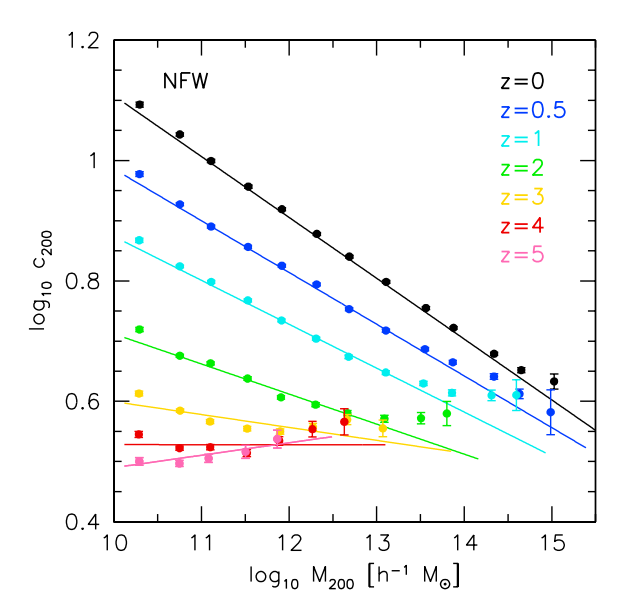
\includegraphics[width=10cm]{images/dutton.png}
\caption[Evolution of the concentration mass relation]{Evolution of the concentration mass relation, by Dutton \& Maccio, \citeyear{Reference23}}
\end{figure}

The surface mass density in the NFW profile is given by:

\begin{equation}
\Sigma_{\text{NFW}}(x) = \left\lbrace
\begin{array}{lll}
\frac{2r_{s}\delta_{c}\rho_{c}}{\left(x^{2}-1\right)}\left[1-\frac{2}{\sqrt{1-x^{2}}}\arctanh\sqrt{\frac{1-x}{1+x}}\right] & (x<1)\\\\
\frac{2r_{s}\delta_{c}\rho_{c}}{3} & (x=1)\\\\
\frac{2r_{s}\delta_{c}\rho_{c}}{\left(x^{2}-1\right)}\left[1-\frac{2}{\sqrt{x^{2}-1}}\arctan\sqrt{\frac{x-1}{1+x}}\right] & (x>1)
\end{array}
\right.
\end{equation} 

so from the critical density:

\begin{equation}
\rho_{c}=\frac{3H^2(z)}{8\pi G}
\end{equation}

$H(z)=H_{0}(1+\Omega z)^{3/2}$

But we are more interested in the enclosed mass which can be done by integrating the surface mass density:

\begin{equation}
\text{M}(R)=\int_{0}^{R}2\pi R\Sigma(R)dR
\end{equation}

The radial dependence on the shear is:

\begin{equation}
\gamma_{\text{NFW}}(x) = \left\lbrace
\begin{array}{lll}
\frac{r_{s}\delta_{c}\rho_{c}}{\Sigma_c}g_{<}(x) & (x<1)\\\\
\frac{r_{s}\delta_{c}\rho_{c}}{\Sigma_c}\left[\frac{10}{3}+4 \ln \left(\frac{1}{2}\right)\right] & (x=1)\\\\
\frac{r_{s}\delta_{c}\rho_{c}}{\Sigma_c}g_{>}(x) & (x>1)
\end{array}
\right.
\end{equation} 

where: 

\begin{equation}
g_{<}(x)=\frac{8 \arctanh \sqrt{\frac{1-x}{1+x}}}{x^{2}\sqrt{1-x^{2}}}+\frac{4}{x^{2}} \ln \left(\frac{x}{2}\right)-\frac{2}{\left(x^{2}-1\right)}+\frac{4 \arctanh \sqrt{\frac{1-x}{1+x}}}{\left(x^{2}-1\right)\left(1-x^{2}\right)^{1/2}}
\end{equation}

\begin{equation}
g_{<}(x)=\frac{8 \arctan \sqrt{\frac{x-1}{1+x}}}{x^{2}\sqrt{x^{2}-1}}+\frac{4}{x^{2}}\ln \left(\frac{x}{2}\right)-\frac{2}{\left(x^{2}-1\right)}+\frac{4 \arctan \sqrt{\frac{x-1}{1+x}}}{\left(x^{2}-1\right){}^{3/2}}
\end{equation}  

\begin{figure}[H]
\centering
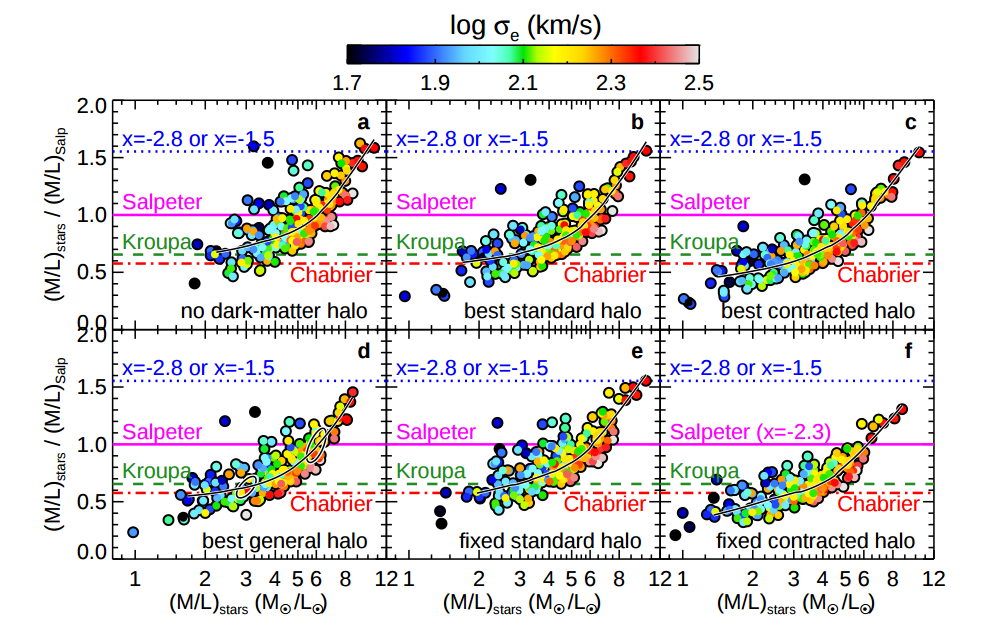
\includegraphics[width=12cm]{images/IMFs_paper.png}
\caption[The systematic variation of the IMF in early-type galaxies.]{The systematic variation of the IMF in early-type galaxies, Cappellari et. al. \citeyear{Reference19}.}
\end{figure}
 
\end{appendices}